\chapter{Irodalmi áttekintés} \label{Research}     
\section{Gyártórendszerek ütemezése}
Ahogyan az már a bevezetésben is említésre került az ütemezési problémák nagy hányadát a gyártásütemezési feladatok teszik ki, melyek elvégzése során a cél általában az átviteli kapacitás, vagy egyszerűen profit (throughput)\footnote{A szakirodalomban általában az angol "throughput" kifejezés a használatos, ha profit maximalizálásról, "makespan", ha idő minimalizálásról van szó, éppen ezért dolgozatomban a továbbiakban én is ezen kifejezések használatára törekszem.} maximalizálása.
Másik fontos célkitűzés lehet a "makespan", vagyis a feladatok elvégzéséhez szükséges idő minimalizálása.
A gyártásütemezési problémák esetében a megoldandó feladatok alatt általában a késztermékek egy részének, összetevőjének a legyártása értendő, az erőforrások, amik között a feladatok kiosztásra kerülnek pedig nem mások mint az elérhető gépek, berendezések, amelyek az adott rész legyártására képesek, adott továbbá az is, hogy melyik berendezés melyik feladatot mennyi idő alatt képes elvégezni, valamint a részfeladatok elvégzésének betartandó sorrendje.
Ezen paraméterek együtt alkotják az un. receptet, mely a feladatok precedenciája alapján a következő kategóriákra bontható:
\begin{itemize}
\item[]\textbf{Single stage recept}: Minden termék egy lépésben állítható elő. 
\item[]\textbf{Simple multiproduct recept:} Minden termék több lineárisan egymást követő lépésből áll elő.
\item[]\textbf{General multiproduct recept}: Az előző fajta speciális esete, ahol a lépések tetszőlegesen kihagyhatóak.
\item[]\textbf{Multipurpose recept}: A lépéseknek nincs meghatározott, lineáris sorrendjük, tetszőleges sorrendben hajthatóak végre.
\item[]\textbf{Precedential recept}: A lépések nem lineárisak, lehetnek elágazások is a lépések között (kör nem lehetséges), egy lépésnek akár több megelőző lépése is lehet, melyek teljesítése a következő lépés megkezdésének a feltétele.
\item[]\textbf{General network recept}: A legáltalánosabb recept kategória, melyben a feladatok a bemenetükkel, illetve a kimenetükkel adottak, indirekt módon meghatározva ezzel a precedenciákat.\cite{hegyhati2010} 
\end{itemize}
A receptek tulajdonságain kívül fontos tényező, különösen vegyi üzemek termelésének ütemezése során a különböző tárolási irányelvek (storage policy) betartása.\cite{phd_Hegyhati}
Tárolási irányelvek alatt azokat a megkötéseket értjük, amelyek a köztes termékek tárolására vonatkoznak a recept két egymást követő feladata között.
A tárolási irányelvek alapvetően két szempont szerint csoportosíthatóak, az egyik az idő, ameddig a köztes termék tárolható anélkül például, hogy bizonyos kémia, fizikai tulajdonságai megváltoznának, amelyre egyébként a következő feladat során szükség lenne (pl. ne hűljön ki a termék).
A másik szempont pedig a mennyiség, azaz, hogy adott köztes termékből adott üzemben mennyit lehet eltárolni.
Ezek alapján a különböző kategóriák azonosíthatóak be:
\begin{itemize}
\item[]\textbf{UW - Unlimited Wait}: A legegyszerűbb, és leggyakoribb eset, melyben a köztes termék bármennyi ideig eltárolható a következő feladat megkezdése előtt.
\item[]\textbf{LW - Limited Wait}: Ebben az esetben a köztes termék nem tárolható egy megadott időnél tovább a következő feladat előtt, hogy ne veszítse el valamilyen tulajdonságát.
\item[]\textbf{ZW - Zero Wait}: Ebben az esetben a köztes termék tárolásának megengedett ideje 0.
\item[]\textbf{UIS - Unlimited Intermediate Storage}: Ebben az esetben végtelen mennyiséget el tudunk tárolni az adott köztes termékből.
\item[]\textbf{FIS - Finite Intermediate Storage}: Az az eset, melyben a köztes termék tárolása megoldható, de véges számú a tároló kapacitás.
\item[]\textbf{NIS - No Intermediate Storage}: Ebben az esetben nem állnak rendelkezésre tároló egységek a köztes termék eltárolására, de a köztes termék továbbra is várakozhat az aktuális feladatot végrehajtó egységben.
\end{itemize}
A recepteken és a tárolási irányelveken kívül a gyártórendszerek ütemezésével kapcsolatos problémák is több szempont szerint is csoportosíthatóak\cite{phd_Hegyhati}:
\begin{itemize}
\item Az ütemezés időpontjában elérhető paraméterek szerint:
\begin{itemize}
\item Offline ütemezésről beszélünk akkor, ha minden szükséges adat rendelkezésre áll az ütemezés megkezdésekor.
\item Online ütemezésnek nevezzük azon eseteket, mikor az ütemezés megkezdésekor még nem minden paraméter áll rendelkezésre, ezért bizonyos paraméterek hiányában kell meghozni az ütemezési döntéseket.
\end{itemize} 
\item A bizonytalanságok alapján:
\begin{itemize}
\item Determinisztikus problémának nevezzük azon eseteket, amelyekben minden paraméter értéke adott már a kidolgozott ütemterv megvalósítása előtt.
\item Sztochasztikus a probléma ezzel szemben, ha valamely paraméter értéke csak az ütemterv végrehajtása során (pl. termelés közben) válik világossá.
\end{itemize}
\end{itemize}
Az ütemezési problémák megoldásai is osztályozhatóak aszerint, hogy a megoldás megvalósítható (feasible), vagy nem valósítható meg (infeasible).
A "megoldás" alatt általában magát az ütemtervet értjük, amely nem más mint az összes feladat hozzárendelése berendezésekhez, illetve időintervallumokhoz.
Infeasible megoldásról akkor beszélünk, ha az ütemterv nem elégíti ki a probléma definiálása során lefektetett megkötések akár egyetlen egy tagját is, ezzel szemben feasible a megoldás, ha az ütemterv minden megkötést kielégít.
A feasible megoldások további csoportját képezik a non-delay megoldások, amelyek esetén egyetlen egy berendezés kapcsán sem beszélhetünk üresjáratról, ha akár csak egy feladat is megvalósításra vár.     
\section{Megoldó módszerek}
Az utóbbi évtizedekben számos különböző módszer került publikálásra, melyek az ütemezési problémák megoldására hivatottak.
Az évek során ezek a módszerek jelentős javuláson mentek keresztül mind a megoldható problémák halmazát tekintve, mind a megoldáshoz szükséges idő gyorsaságát figyelembe véve.
A következő alpontokban néhány megoldó módszer kerül megemlítésre.
\subsubsection{MILP modellek}
A publikációk túlnyomó része matematikai programozáson, név szerint a Mixed-Integer Linear Programming, azaz MILP modelleken alapszik.
A modellek általában univerzális MILP algoritmusokkal kerülnek megoldásra. \cite{9780471283669}
A MILP modelleknek különböző típusai léteznek:
\begin{description}
\item[\textbf{Időfelosztásos módszerek (Time discretization based)}]: Az időhorizont diszkrét pontokra, vagy résekre bontásán alapszanak, mely szuboptimális, vagy akár infeasible megoldáshoz is vezethet, azonban ezen módszerek segítségével az ütemezési problémák széles skálája valósítható meg.
Időrendi szempontból ezen modellek jelentek meg először a szakirodalomban. \cite{KONDILI1993211}
Minden időpontban bináris változók vannak hozzárendelve a feladatokhoz, melyek értéke jelenti, hogy adott feladat végrehajtása az adott időpontban kezdődik el vagy sem.
Jól látható, hogy a változók száma arányos a kiválasztott időpontok számával, ezáltal az ütemezés teljesítéséhez szükséges számítási idő nagyban függ a diszkrét időpontok számától, éppen ezért mindig is kutatási szándék volt olyan módszer fejlesztése, amely képes az optimális megoldás meghatározására minimális diszkrét időpont alapján.
\item[\textbf{Precedencia alapú módszerek (Precedence based)}]: Az időfelosztásos módszerekkel szemben a precedencia alapú módszerek esetén nincs szükség az időhorizont diszkretizációjára, ezáltal nem használnak ismeretlen paramétereket a megoldás során.
A megoldható problémák halmaza kisebb mint az előző típus esetében, azonban a megoldható problémákra alapvetően jobb megoldást szolgáltatnak a precedencia alapú módszerek.
A legtöbb modell multiproduct és multipurpose receptekre lett bevezetve, azonban többségük egyszerűen kibővíthető, hogy általánosabb problémák megoldására is használható legyen.
A módszerek alapja két különböző bináris változó halmaz: $Y_{i,j}$, melynek értéke 1, ha $i$ feladatot $j$ berendezéshez rendeljük, valamint $X_{i,j,i'}$, mely akkor vesz fel 1 értéket, ha $i$ és $i'$ feladatokat egyaránt $j$ berendezéshez rendeljük, méghozzá úgy, hogy $i$ elvégzése megelőzi $i'$ elvégzését $j$ berendezésen. 
\end{description}
\subsubsection{Időzített automaták, Időzített Petri háló}
A Petri hálók, és automaták gyakran használatosak diszkrét eseményrendszerek modellezésére, ahhoz azonban, hogy ezen módszerek felhasználhatóak legyenek gyártásütemezési problémák megoldására is, időzítésekkel kellett kiegészíteni őket.
Így születtek meg a Timed Place Petri Nets (TPPN), Timed Priced Automata (TPA) módszerek.
Ezen módszerek Branch \& Bound algoritmust használnak az állapottér bejárására, és a legkedvezőbb megoldás megtalálására.
A hatékony modellezésnek köszönhetően a modellezési hibák könnyen kikerülhetőek, valamint a módszer könnyen kibővíthető a reaktív ütemezési feladatok kezelésére is, ennek ellenére azonban ezen módszerek hatékonysága elmarad a MILP modellek, illetve az S-gráf modell hatékonyságától is.  
\subsubsection{S-gráf keretrendszer}
Az S-gráf keretrendszer, amely ezen szakdolgozat fő fókuszát képezi, volt az első publikált gráf elméleten alapuló módszer szakaszos gyártórendszerek ütemezésére.
Az S-gráf keretrendszer részletesebb bemutatása a \ref{S-graph}. fejezetben olvasható. 
\section{Az ütemtervek vizualizációja}
Az ütemezési problémák megoldása során keletkezett ütemterveket Gannt-diagrammal szokás ábrázolni, mely nevét feltalálójáról Henry Gantt amerikai mérnökről kapta. \cite{0879600489}
Az ütemtervek lényegében a következő formájú négyesekből állnak: ($i,j,t^s,t^f$), ahol
\begin{itemize}
\item[$i$] az elvégzendő feladat
\item[$j$] az $i$ feladatot elvégző berendezés
\item[$t^s$] a feladat elvégzésének kezdeti időpontja
\item[$t^f$] a feladat elvégzésének vég időpontja
\end{itemize}
\begin{figure}[H]
\begin{center}
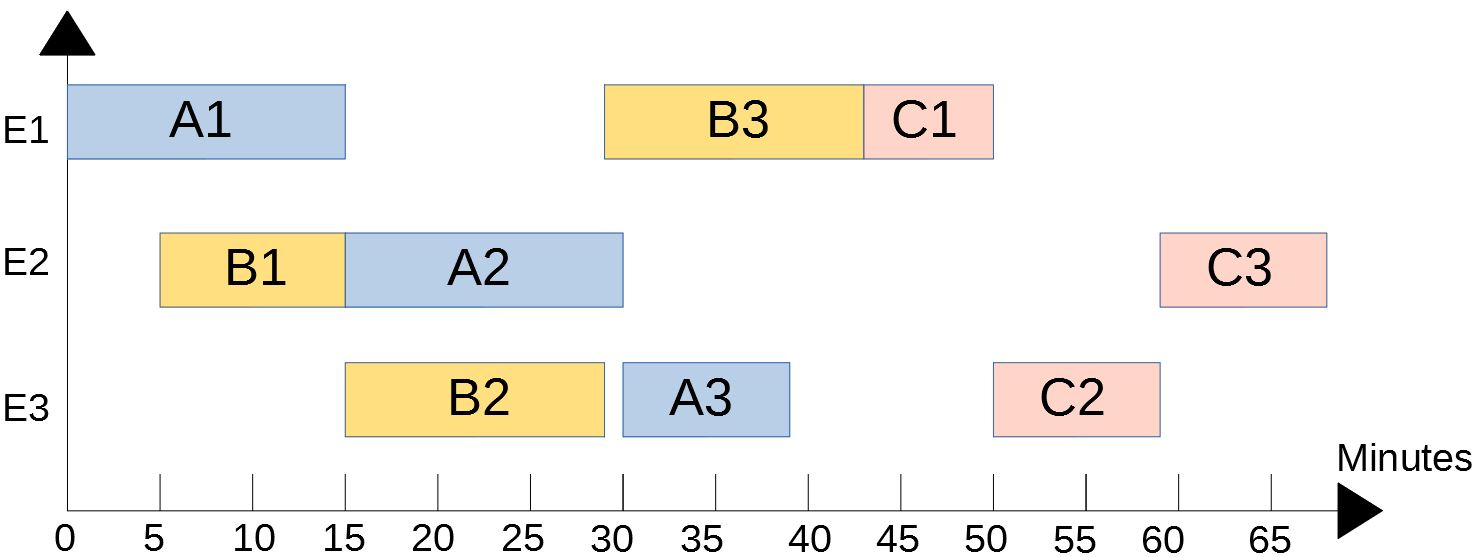
\includegraphics[scale=0.375]{gannt}
\caption{Gannt-diagram egy ütemterv szemléltetésére}
\label{gannt}
\end{center}
\end{figure}
Egy Gannt-diagram szemléltetésére szolgál a \ref{gannt} ábra.
Látható, hogy az $y$ tengelyen a berendezések nevei (E1,E2,E3) találhatóak, míg az $x$ tengely az idő szemléltetésére hivatott.
Az ábra három különböző termék (A,B,C), valamint azok részfeladatainak ütemezését szemlélteti, melyeket különböző színekkel jelölünk.
A Gannt-diagramos ábrázolás segítségével az ütemtervet képező négyesek minden paramétere egyszerűen leolvasható.
Az elvégzendő feladat neve a színes téglalapokon találhatóak (pl. C1), a feladatot elvégző berendezést az adott téglalap $y$ tengelyen vett helye határozza meg (pl. C1 esetében E1 berendezés).
A feladatok elvégzésének a kezdeti, illetve vég időpontja pedig az téglalapok $x$ tengelyen vett helye alapján könnyen beazonosíthatóak, meghatározva ezáltal a feladat teljesítéséhez szükséges időt is. 